%
% Differenzierbare Zerlegungen der Einheit
%
\section{Differenzierbare Zerlegung der Einheit
\label{buch:kurvenintegral:section:zerlegung}}
Ein Wegintegral kann sich entlang eines Pfades erstrecken, der
mehrere Kartengebiete einer Mannigfaltigkeit durchschneidet.
Das Kurvenintegral ist mithilfe eines Koordinatensystems definiert,
kann also immer nur innerhalb eines Kartengebietes
mit einem Riemann-Integral berechnet werden.
Es muss also ein Technik gefunden werden, mit der Teilintegrale in
einzelnen Kartengebieten zu einem Integral über die ganze Kurve
zusammengesetzt werden.
Die Konstruktion muss von der Wahl der Koordinatensysteme entlang
des Pfades unabhängig sein.
Dies wird erreicht mit einer differenzierbaren Zerlegung der Einheit
und ist möglich dank der Tatsache, dass das Kurvenintegral linear
in der 1-Form ist.

\kopfrechts{Differenzierbare Zerlegung der Einheit}%

%
% Glatte Funktionen mit Träger in einem Interval
%
\subsection{Glatte Funktionen mit Träger in einem Interval}
Wir müssen eine beliebig oft differenzierbare Funktion konstruieren,
die genau auf einem vorgegebenen offenen Intervall von Null
verschieden ist.

%
% Der Träger einer Funktion
%
\subsubsection{Der Träger einer Funktion}
Der Träger einer Funktion ist die Teilmenge des Definitionsbereichs,
auf dem die Funktion nicht verschwindet.
Genauer gilt die folgende Definition.

\begin{definition}[Träger einer Funktion]
Sei $f\colon M\to\mathbb{R}$ eine differenzierbare Funktion.
Der \emph{Träger} von $f$ ist die Menge
\index{Trager@Träger}%
\index{Trager@Träger}%
\index{supp}%
\[
\operatorname{supp}(f)
=
\overline{
\{x\in M\mid f(x)\ne 0\}
},
\]
der Abschluss der Menge der Punkte, in denen $f$ von $0$ verschieden
ist.
\end{definition}

Nimmt man beliebige Mengen $U$, auf denen die Funktion $f$ verschwindet,
dann ist die Vereinigung dieser Mengen $U$ das Komplement des Trägers
und auch wieder eine offene Menge.
Ein Punkt im Komplement des Trägers enthält also immer eine kleine
Umgebung, auf der die Funktion $f$ verschwindet.

%
% Eine glatte Funktion mit Träger $\mathbb{R}_{\ge 0}$
%
\subsubsection{Eine glatte Funktion mit Träger $\mathbb{R}_{\ge 0}$}
%
% fig-e1x.tex
%
% (c) 2025 Prof Dr Andreas Müller
%
\begin{figure}
\centering
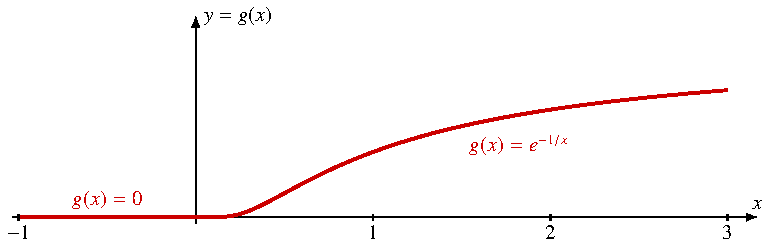
\includegraphics{chapters/030-kurvenintegral/images/e1x.pdf}
\caption{Die Funktion $g(x)$ ist beliebig oft stetig differenzierbar
und hat $\mathbb{R}_{\ge 0}$ als Träger.
\label{buch:kurvenintegral:fig:e1x}}
\end{figure}
%
Die Funktion
\[
g(x)
=
\begin{cases}
e^{-1/x}&\qquad \text{für $x>0$}\\
0       &\qquad \text{sonst.}
\end{cases}
\]
ist sicher beliebig oft differenzierbar ausserhalb des Punktes $x=0$
(Abbildung~\ref{buch:kurvenintegral:fig:e1x}).
Die linksseitigen Ableitungen der Funktion im Punkt $0$ verschwinden
alle.
Es ist also zu überprüfen, ob auch die rechtsseitigen Ableitungen
verschwinden.
Dazu berechnen wir die Ableitungen von $e^{-1/x}$ mit Hilfe der
Kettenregel:
\begin{align*}
\frac{d}{dx}e^{-1/x}
&=
e^{-1/x}\frac{d}{dx}\biggl(-\frac1x\biggr)
=
e^{-1/x}\frac{1}{x^2}
\\
\end{align*}


\begin{satz}
Die $k$-te Ableitung der Funktion $f(x)=e^{-1/x}$ ist von der Form
\[
\frac{d^n}{dx^n}f(x)
=
f^{(n)}(x)
=
\frac{P_n(x)}{x^{2n}}e^{-1/x},
\]
wobei $P_n(x)$ ein Polynom vom Grad $n-1$ ist, welches die
Rekursionsformel
\[
P_{n+1}(x)
=
x^2P'_n(x) + (1-2nx)P_n(x)
\]
erfüllt.
\end{satz}

\begin{proof}
Die Aussage kann mithilfe von vollständiger Induktion bewiesen
werden.
Sie ist offensichtlich für die $0$-te Ableitung, also für die Funktion
$f(x)$ selbst war, das Polynom $P_0(x)=1$ ist als Konstante vom Grad 0.

Um den Induktionsschritt durchzuführen, nehmen wir an, dass $f^{(n)}(x)$
die behauptete Form hat, und berechnen die Ableitung
\begin{align}
f^{(n+1)}(x)
&=
\frac{d}{dx}
f^{(n)}(x)
=
\frac{d}{dx}
\frac{P_n(x) e^{-1/x}}{x^{2n}}
\notag
\\
&=
\frac{P'_n(x)e^{-1/x}}{x^{2n}}
+
\frac{P_n(x)e^{-1/x}}{x^{2n}}\frac{d}{dx}\biggl(-\frac1x\biggr)
+
P_n(x)e^{-1/x}\frac{d}{dx}\frac{1}{x^{2n}}
\notag
\\
&=
\Bigl(
x^2 P'_n(x)
+
P_n(x)
-
2nx P_n(x)
\Bigr)\frac{e^{-1/x}}{x^{2(n+1)}}
\notag
\\
&=
\Bigl(x^2P'_n(x)+(1-2nx)P_n(x)\Bigr) \frac{e^{-1/x}}{x^{2(n+1)}}.
\label{buch:kurvenintegral:zerlegung:eqn:rekursion}
\end{align}
Die Ableitung $P'_n(x)$ ist ein Polynom vom Grad $n-2$, also ist
$x^2P'_n(x)$ vom Grad $n$.
Ebenso ist der zweite Summand $(1-2nx)P_n(x)$ in
\eqref{buch:kurvenintegral:zerlegung:eqn:rekursion}
ein Polynom vom Grad $n$.
Das Polynom
\[
P_{n+1}(x)
=
x^2P'_{n}(x)+(1-2nx)P_n(x)
\]
ist das gesuchte Polynom.
\end{proof}

\begin{satz}
\label{buch:kurvenintegral:zerlegung:satz:g}
Die Funktion
\[
g(x)
=
\begin{cases}
e^{-1/x}&\qquad\text{für $x>0$}\\
0&\qquad\text{sonst}
\end{cases}
\]
ist beliebig oft stetig differenzierbar.
\end{satz}

\begin{proof}
Es ist bereits bekannt, dass die Funktion stetig differenzierbar ist
ausserhalb des Punktes $x=0$.
Es muss also nur noch gezeigt werden, dass alle Ableitungen von $f$
für $x\to 0$ gegen $0$ konvergieren.
Dazu berechnet man
\begin{align}
\lim_{x\to 0+} f^{(n)}(x)
&=
\lim_{x\to 0+} P_n(x) \frac{e^{-1/x}}{x^{2n}}.
\notag
\intertext{Als Polynom ist $P_n(x)$ stetig an der Stelle $0$,
sein Grenzwert für $x\to 0$ ist $P_n(0)$.
Der Grenzwert der Ableitung kann damit vereinfacht werden zu}
&=
P_n(0) \lim_{x\to 0+}\frac{e^{-1/x}}{x^{2n}}.
\notag
\intertext{Schreibt man $x=1/t$, wird daraus der Grenzwert}
&=P_n(0)\lim_{t\to\infty}t^{2n}e^{-t}
\label{buch:kurvenintegral:zerlegung:eqn:bruch}
\end{align}
für $t\to\infty$.
Der Kehrwert des Bruchs in
\eqref{buch:kurvenintegral:zerlegung:eqn:bruch}
ist
\begin{align*}
\lim_{t\to\infty}
\frac{1}{t^{2n}e^{-t}}
&=
\lim_{t\to\infty}
\frac{u(t)}{v(t)}
=
\lim_{t\to\infty}
\frac{e^t}{t^{2n}}
=
\lim_{t\to\infty},
\intertext{auf den die Regel von de l'Hospital für den Bruch $u(t)/v(t)$
mit $u(t)=e^t$ und $v(t)=t^{2n}$ wiederholt angewendet werden kann.
Die Ableitungen von $u$ sind $u^{(k)}(t)=e^t$ und
$v^{(k)}=2n(2n-1)\dots(2n-k+1)x^{2n-k}$.
$2n$-malige Anwendung ergibt daher}
\lim_{t\to\infty}
\frac{1}{t^{2n}e^{-t}}
&=
\lim_{t\to\infty}\frac{u^{(2n)}(t)}{v^{(2n)}(t)}
=
\lim_{t\to\infty}\frac{e^t}{(2n)!}=\infty.
\end{align*}
Dies zeigt, dass der Grenzwert
\eqref{buch:kurvenintegral:zerlegung:eqn:bruch}
verschwindet.
\end{proof}

%
% Eine glatte Funktion mit Trägerr [a,b]
%
\subsubsection{Eine glatte Funktion mit Träger $[a,b]$}
Mit der Funktion $g(x)$ von Satz~\ref{buch:kurvenintegral:zerlegung:satz:g}
lässt sich jetzt eine beliebig oft stetig differnzierbare
Funktion mit Träger im Intervall $[a,b]$ konstruieren.

%
% fig-gab.tex
%
% (c) 2025 Prof Dr Andreas Müller
%
\begin{figure}
\centering
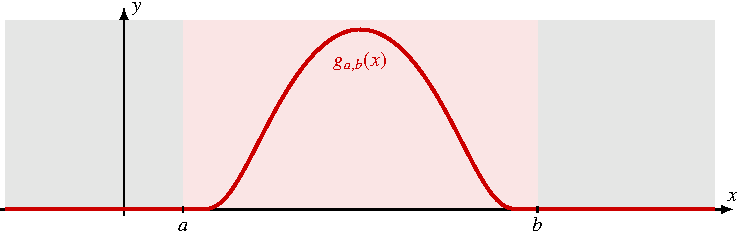
\includegraphics{chapters/030-kurvenintegral/images/gab.pdf}
\caption{Die Funktion $g_{a,b}(x)$ ist beliebig of stetig differenzierbar
und hat das abgeschlossene Intervall $[a,b]$ als Träger,
der durch das hellrote Hintergrundrechteck dargestellt wird.
\label{buch:kurvenintegral:fig:gab}}
\end{figure}
%

\begin{satz}
Für $a,b\in\mathbb{R}$ mit $a<b$ ist
die Funktion
\[
g
\colon
\mathbb{R}\to\mathbb{R}
:
x\mapsto
g_{a,b}(x)
=
g(x-a)\cdot g(b-x)
\]
beliebig oft stetig differenzierbar und hat Träger $[a,b]$.
\end{satz}

\begin{proof}
Für $x<a$ ist $x-a<0$ und daher $g(x-a)=0$.
Für $x>b$ ist $b-x<0$ und daher $g(b-x)=0$.

Für $x$ im offenen Intervall $(a,b)$ ist $x-a>0$ und $b-x>0$, daher ist
$g(x-a)>0$ und $g(b-x)>0$ und damit
auch $g_{a,b}(x)=g(x-a)g(b-x)>0$.
Damit ist gezeigt, dass $g_{a,b}(x)\ne 0$ für $x\in(a,b)$ und damit
\[
\operatorname{supp} g_{a,b}(x)
=
[a,b],
\]
wie behauptet.
\end{proof}

Der Graph der Funktion $g_{a,b}(x)$ ist in
Abbildung~\ref{buch:kurvenintegral:fig:gab}
mit stark gestreckter vertikaler Skala dargestellt.
Der Träger ist als hellrotes Rechteck hervorgehoben.

%
% Überdeckung mit offenen Intervallen
%
\subsection{Überdeckung mit offenen Intervallen}
Eine Kurve auf einer $n$-dimensionalen Mannigfaltigkeit kann sich
nacheinander durch mehrere Kartengebiet winden.
In jedem Kartengebiet lässt sich eine auf der Mannigfaltigkeit
definierte $1$-Form $\alpha$ in den Koordinaten ausdrücken und das
Integral kann mit den Methoden der klassischen Integralrechnung
berechnet werden.
Damit wird aber der Beitrag zum Integral ausserhalb der Karte
ignoriert und es ist unklar, was am Rande des Kartengebietes
passiert.

Sei $[a,b]$ das Parametergebiet der Kurve $\gamma\colon\mathbb{R}\to M$,
welches in eine einzige Karte abgebildet wird.
Die 1-Form $g_{a,v}(x)(T\gamma)_*\alpha(x)$ verswindet ausserhalb
des Intervalls $[a,b]$, so dass das Integral über die Kurve nur
vom Teil im Inneren der Karte abhängt.
Damit besteht die Möglichkeit, das Integral von $\alpha$ über
die ganze Kurve zusammenzusetzen aus Summanden, die jeweils nur
innerhalb eines Kartengebietes von $0$ verschieden sind.
Zusätzlich sollten jeweils nur endlich viele Summanden gleichzeitig
von 0 verschieden sein, da sonst auch noch ein Begriff des Grenzwertes
einer unendlichen Summe von 1-Formen definiert werden müsste.
Es muss also untersucht werden, ob es möglich ist, aus einer
Überdeckung des Definitionsbereichs der Kurve durch offene Intervalle
eine Überdeckung auszuwählen, die jeden Punkt des Definitionsgebietes
nur in endlich vielen Mengen enthält.

\begin{satz}
\label{buch:kurvenintegral:zerlegung:satz:kompakt}
Sei $U_\alpha \subset [a,b]$, $\alpha\in I$, eine Familie offener
Intervalle in $\mathbb{R}$, die die ganze Menge $[a,b]$ überdecken,
also
\[
\bigcup_{\alpha\in I} U_\alpha \supset [a,b].
\]
Dann gibt es eine endliche Teilmenge $J\subset I$ derart, dass
\[
\bigcup_{\alpha\in J}U_\alpha\supset [a,b].
\]
\end{satz}

\begin{proof}
Wir beweisen die Aussage mithilfe eines Widerspruchs.
Wir nehmen also an, dass in jeder Vereinigung von endlich vielen
der Mengen $U_\alpha$ mindestens ein Punkt von $[a,b]$ nicht
enthalten ist.
Wir führen dies zu einem Widerspruch.

Als ersten Schritt dürfen wir annehmen, dass die Familie $I$ abzählbar
unendlich ist.
Die Menge der rationalen Zahlen im Intervall $[a,b]$ ist nämlich
abzählbar.
Indem wir zu jeder rationalen Zahl in $[a,b]$ eine der Mengen $U_\alpha$
auswählen, die die Zahl enthält, erhalten wir eine abzählbare Familie
von offenen Intervallen, die alle rationalen Zahlen in $[a,b]$
enthalten.
Da die rationalen Zahlen dicht sind im Intervall $[a,b]$, muss die
Vereinigung der Intervalle ganz $[a,b]$ enthalten.
Wir nehmen daher im folgenden an, dass $I=\mathbb{N}$ ist.

Nach Voraussetzung gibt es zu jeder natürlichen Zahl $n$ ein
\begin{equation}
x_n \in [a,b] \setminus \bigcup_{i=1}^n U_i.
\label{buch:kurvenintegral:zerlegung:eqn:xn}
\end{equation}
Die Folge $x_n$ ist beschränkt und enthält daher eine konvergente
Teilfolge, die gegen $x=\lim_{n\to\infty}x_n\in[a,b]$ konvergiert.
Da die Gesamtheit der $U_i$ das Intervall $[a,b]$ überdecken, gibt
es ein $n$ derart, dass $x\in U_n$.
Da $x$ der Grenzwert einer Teilfolge von $x_n$ ist, müssen unendlich
viele Punkte der Folge in $U_n$ sein, was der Konstruktion
\eqref{buch:kurvenintegral:zerlegung:eqn:xn}
von $x_n$ widerspricht.
Der Widerspruch zeigt, dass sich $[a,b]$ mit endlich vielen
Mengen der Familie überdecken lässt.
\end{proof}

Die in Satz~\ref{buch:kurvenintegral:zerlegung:satz:kompakt}
formulierte Eigenschaft ist als {\em Kompaktheit} bekannt.

\begin{definition}[Kompaktheit]
Ein topologischer Raum heisst {\em kompakt}, wenn jede Familie
\index{kompakt}%
offener Teilmenge, die den Raum überdecken, eine endliche Teilfamilie
enthält, die den Raum ebenfalls überdecken.
\end{definition}

Kompaktheit ist also genau die Endlichkeitsbedingung, die wir benötigen
um sicherzustellen, dass wir nur jeweils endlich viele Summanden
zusammenfügen müssen.

%
% Differenzierbre Zerlegung der Einheit
%
\subsection{Differenzierbare Zerlegung der Einheit
\label{buch:kurvenintegral:zerlegug:subsection:dze}}
Sei $M$ eine $n$-dimensionale Mannigfaltigkeit mit einem Atlas mit
den Kartengebieten $U_\alpha$, $\alpha\in I$.
Sei ausserdem $\gamma\colon [a,b]\to M$ eine differenzierbare
Kurve in $M$.
Die Mengen
\[
V_\alpha
=
\gamma^{-1}(U_\alpha)
=
\{
t\in[a,b]
\mid
\gamma(t)\in U_\alpha
\}
\]
sind offene Teilmengen von $[a,b]$.
Sie müssen nicht notwendigerweise zusammenhängend sein, die Kurve kann
das Gebiet $U_\alpha$ mehrmals verlassen und wieder neu betreten.
Jedes $V_\alpha$ kann wieder zerlegt werden in endlich viele Intervalle.
Damit ist eine Familie von offenen Intervallen gefunden, die ganz
$[a,b]$ abdecken.

Die Kompaktheit von $[a,b]$ bedeutet, dass es auch eine endliche
Familie von Mengen $V_i$, $i=1,\dots,N$ gibt mit der Eigenschaft,
dass
\[
\bigcup_{i=1}^N V_i = [a,b].
\]
Jede der Mengen $V_i$ ist ein Intervall $V_i=(a_i,b_i)$.
Die Funktionen $g_i(x) = g_{a_i,b_i}(x)$ ist genau in $V_i$
von $0$ verschieden.
Da die Intervalle $V_i$ ganz $[a,b]$ überdecken, ist die
Summe
\begin{equation}
G(x) = \sum_{i=1}^N g_i(x) \ne 0
\label{buch:kurvenintegral:zerlegung:eqn:sum}
\end{equation}
für alle $x\in[a,b]$.
Da es auserdem nur endlich viele Funktionen gibt, hat die Summe
\eqref{buch:kurvenintegral:zerlegung:eqn:sum}
nur endlich viele Summanden, es gibt keine offenen Fragen der
Konvergenz.

Da die Funktion $G(x)$ beliebig oft stetig differenzierbar ist
und nirgends verschwindet, ist auch $1/G(x)$ beliebig oft stetig
differenzierbar.
%
% fig-zerlegung.tex
%
% (c) 2025 Prof Dr Andreas Müller
%
\begin{figure}
\centering
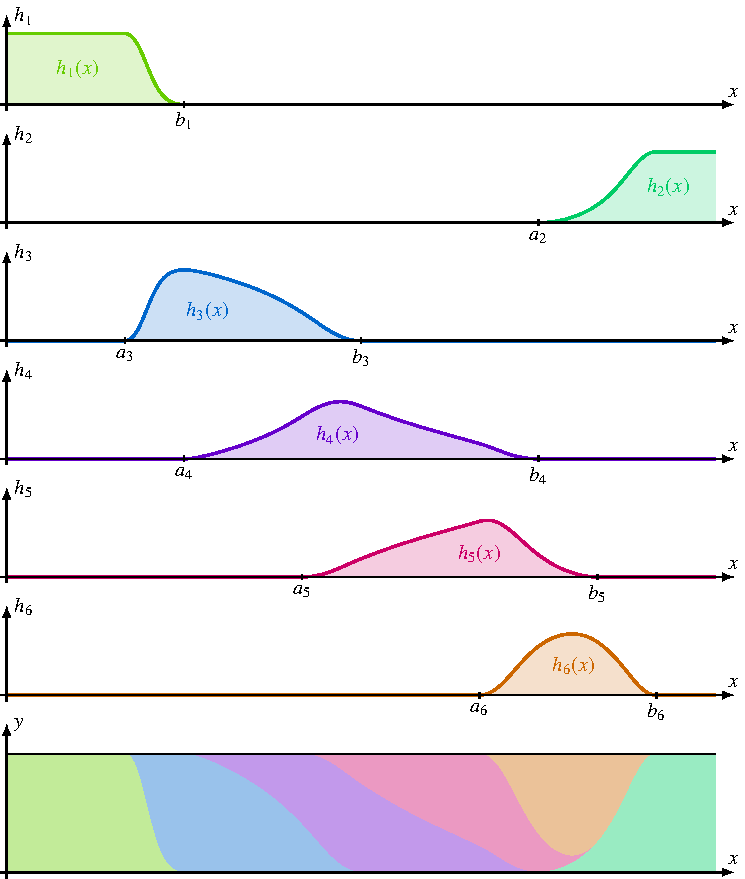
\includegraphics{chapters/030-kurvenintegral/images/zerlegung.pdf}
\caption{Zerlegung der Einheit mit sechs Intervallen $[a_i,b_i]$,
ermittelt mit der Methode dieses Kapitels.
Zunächst wurden die Funktionen $g_i = g_{a_i,b_i}$ konstruiert, dann
wurden die Funktionen $h_i$ durch Normierung mit der Summe der $g_i$
gewonnen.
Die unterste Graphik zeigt, wie die funktionen zusammen wieder den
Wert $1$ ergeben.
\label{buch:kurvenintegral:fig:zerlegung}}
\end{figure}
%
Damit können die neuen Funktion
\[
h_i(x)
=
\frac{1}{G(x)}\,g_i(x)
=
\frac{1}{G(x)}\,g_{a_i,b_i}(x)
\]
definiert werden.
Jede Funktion $h_i(x)$ ist beliebig oft stetig differenzierbar und
es gilt
\[
\sum_{i=1}^N h_i(x)
=
\frac{1}{G(x)}
\underbrace{\sum_{i=1}^N g_i(x)}_{\displaystyle=G(x)}
=
1.
\]
Die Funktionen $h_i(x)$ bilden was man eine {\em Zerlegung der Einheit}
nennt.
\index{Zerlegung der Einheit}%
Dieses Vorgehen zur Gewinnung einer Zerlegung der Einheit ist auch
in Abbildung~\ref{buch:kurvenintegral:fig:zerlegung} illustriert.

%
% Zerlegung eines Kurvenintegrals
%
\subsection{Zerlegung eines Kurvenintegrals}
Sei $\omega$ eine 1-Form auf der $n$-dimensionalen Mannigfaltigkeit $M$,
$\gamma\colon[a,b]\to M$ eine Kurve in $M$
und seien die Funktionen $h_i(x)$ eine Zerlegung der Einheit wie in
Abschnitt~\ref{buch:kurvenintegral:zerlegug:subsection:dze} konstruiert.
Auf jeder Menge $V_i$ lässt sich die 1-Form $(T\gamma)_*(\omega)$ mit
Hilfe einer Karte berechnen.
Die 1-Form
\[
\omega_i
=
h_i\, (T\gamma)^*(\omega)
\]
verschwindet ausserhalb des Intervalls $V_i=[a_i,b_i]$.
Die Summe ist
\[
\sum_{i=1}^N \omega_i
=
\sum_{i=1}^n
h_i\, (T\gamma)^*(\omega)
=
(T\gamma)^*
\sum_{i=1}^n h_i\,
\omega
=
(T\gamma)^*
\biggl(
\sum_{i=1}^n h_i
\biggr)
\omega
=
(T\gamma)^*\omega.
\]
Das Integral entlang der Kurve ist daher
\[
\int_\gamma \omega_i
=
\int_{a_i}^{b_i} h_i(x(t)) \langle \omega(x), \dot{x}(t)\rangle\,dt.
\]
Das Integral von $\omega$ kann jetzt in eine Summe von Integralen
zerlegt werden, die einzeln in einer Karte berechnet werden können:
\[
\int_\gamma\omega
=
\sum_{i=1}^N \int_{\gamma} \omega_i.
\]
Eine differenzierbare Zerlegung der Einheit ermöglich also, jedes
Kurvenintegral auf differenzierbare Art in Integrale innerhalb
einer Karte zu zerlegen.
Damit ist sichergestellt, dass das Integral einer $1$-Form
auf einer Kurve einen Sinn unabhängig davon hat, wie die Mannigfaltigkeit
mit Karten überdeckt wird.

